\documentclass[11pt,oneside]{book}
\usepackage[T1]{fontenc}
\usepackage[utf8]{inputenc}
\usepackage{lmodern}
\usepackage[a4paper,margin=26mm,headheight=15pt]{geometry}
\usepackage{microtype}
\usepackage{setspace}
\usepackage{amsmath,amssymb,mathtools}
\usepackage{booktabs,longtable,tabularx,array,multirow}
\usepackage{graphicx}
\usepackage{float}
\usepackage[dvipsnames,table]{xcolor}
\usepackage{tikz}
\usetikzlibrary{arrows.meta,positioning,fit,backgrounds,shapes.geometric}
\usepackage{pgfplots}
\pgfplotsset{compat=1.18}
\usepackage{enumitem}
\usepackage{fancyhdr}
\usepackage{titlesec}
\usepackage{csquotes}
\usepackage[numbers,sort&compress]{natbib}
\usepackage[hidelinks]{hyperref}
\usepackage[nameinlink,noabbrev]{cleveref}

\definecolor{TrustBlue}{HTML}{0B5FFF}
\definecolor{TrustNavy}{HTML}{10233F}
\definecolor{TrustViolet}{HTML}{6A42D8}
\definecolor{TrustGreen}{HTML}{178A63}
\definecolor{TrustOrange}{HTML}{DB6B26}
\definecolor{TrustLight}{HTML}{F2F6FC}
\definecolor{TrustGray}{HTML}{5D6876}

\hypersetup{
  pdftitle={Identity Trust and Inclusion Fabric},
  pdfauthor={Guillaume Harbonnier},
  pdfsubject={Executive Master Thesis and Industrial Product Proposal},
  pdfkeywords={identity, biometrics, verifiable credentials, anomaly detection, graph neural networks, inclusion}
}

\pagestyle{fancy}
\fancyhf{}
\fancyhead[L]{\small Identity Trust \& Inclusion Fabric}
\fancyfoot[C]{\thepage}
\renewcommand{\headrulewidth}{0.3pt}
\titleformat{\chapter}[display]{\bfseries\color{TrustNavy}}{\filleft\Large\chaptername\ \thechapter}{1ex}{\titlerule\vspace{1ex}\Huge}
\titleformat{\section}{\Large\bfseries\color{TrustNavy}}{\thesection}{0.7em}{}
\titleformat{\subsection}{\large\bfseries\color{TrustBlue}}{\thesubsection}{0.7em}{}
\setstretch{1.17}
\setlength{\parskip}{0.45em}
\setlength{\parindent}{0pt}
\setlist{nosep,leftmargin=1.7em}
\newcolumntype{Y}{>{\raggedright\arraybackslash}X}

\newcommand{\product}{Identity Trust \& Inclusion Fabric}
\newcommand{\claimboundary}{\textbf{Claim boundary.} All experimental data and reported proof-of-function results are synthetic. They do not estimate operational fraud, biometric, fairness, or inclusion performance.}
% Generated by scripts/run_experiment.py; do not edit by hand.
\newcommand{\TestN}{3,461}
\newcommand{\FraudRate}{5.37\%}
\newcommand{\RocAuc}{1.000}
\newcommand{\AvgPrecision}{0.998}
\newcommand{\Brier}{0.0383}
\newcommand{\RecallCapacity}{100.0\%}
\newcommand{\ReviewCapacity}{12.0\%}
\newcommand{\NovelRecall}{100.0\%}
\newcommand{\ExclusionAuc}{0.987}


\begin{document}

\begin{titlepage}
\pagecolor{TrustNavy}
\color{white}
\vspace*{18mm}
{\Large EXECUTIVE MASTER THESIS AND INDUSTRIAL PRODUCT PROPOSAL\par}
\vspace{15mm}
{\Huge\bfseries Identity Trust \& Inclusion Fabric\par}
\vspace{5mm}
{\LARGE Beyond the Matcher: Federated Assurance for Biometrics, Credentials, Fraud, and Inclusive Access\par}
\vfill
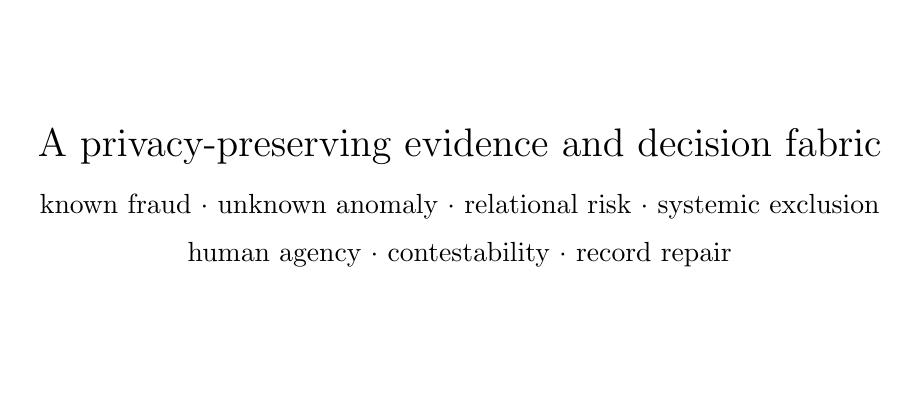
\begin{tikzpicture}
\node[draw=white,rounded corners=5pt,minimum width=\textwidth-15mm,minimum height=43mm,align=center,line width=0.7pt] {
\Large A privacy-preserving evidence and decision fabric\\[3mm]
\normalsize known fraud $\cdot$ unknown anomaly $\cdot$ relational risk $\cdot$ systemic exclusion\\[2mm]
\normalsize human agency $\cdot$ contestability $\cdot$ record repair
};
\end{tikzpicture}
\vfill
{\Large Guillaume Harbonnier\par}
{\large Version 0.1.0 --- Research Draft --- 19 July 2026\par}
\vspace{8mm}
{\small Not peer reviewed. Synthetic research demonstrator. No operational use without customer-specific validation, lawful governance, and independent review.\par}
\end{titlepage}
\nopagecolor
\color{black}

\frontmatter
\chapter*{Abstract}
\addcontentsline{toc}{chapter}{Abstract}

Identity ecosystems are assembled from capable but fragmented components: biometric matchers, presentation-attack detection, document inspection, authoritative registries, digital wallets, credential issuers, rules, fraud platforms, and human investigators. Yet the architecture often retains an uninstantiated box labelled \emph{Fraud Detection}. It has no agreed threat ontology, evidence contract, decision authority, feedback loop, or measure of harm to legitimate people. This thesis asks how that empty box can become a governed industrial capability without becoming a surveillance platform.

We propose the \product: a federated, purpose-bound evidence and decision layer spanning public authorities, private biometric suppliers, telecommunications operators, professional credential issuers, relying parties, and citizens. It combines four complementary signals: supervised detection of known fraud, density- or isolation-based detection of novel anomalies, graph-based relational risk, and process anomaly detection for systemic exclusion. The output is not a universal citizen score and not an automatic accusation. It is a transaction-specific, calibrated assessment that selects the least intrusive effective action: approve, monitor, request additional evidence, allocate human expertise, or escalate under explicit policy.

The research extends four earlier lines of work: \emph{Beyond the Matcher}, a calibrated human--AI multibiometric decision and remedy framework; a Biometric Fraud Simulation Framework using synthetic scenarios, a Matcher Mock, a real matcher phase, and a truth matrix; a National Identity Fraud Risk Engine using identity--device--IP graphs and GNNs; and anomaly detection as open-set modelling of normal behaviour. The extension introduces a trust ontology for verifiable credentials, issuer and holder relationships, a co-equal anti-exclusion objective, deterministic redress and record repair, and a product architecture designed for sovereign or on-premise deployment.

A reproducible synthetic proof of function is provided. It generates score-level biometric, credential, device, graph, and process events; temporally separates train and test data; withholds a class of novel fraud from supervised learning; and evaluates a hybrid random forest, Isolation Forest, relational reuse score, and process-exclusion detector. On a synthetic temporal test set of \TestN{} events, the hybrid reaches ROC AUC \RocAuc{}, average precision \AvgPrecision{}, and \RecallCapacity{} fraud recall at a \ReviewCapacity{} review capacity. Novel-fraud recall is \NovelRecall{}, while the exclusion detector reaches ROC AUC \ExclusionAuc{}. These figures establish pipeline executability only. They do not constitute product-performance claims.

The industrial conclusion is conditional but positive. The market already contains strong component and platform offers; novelty cannot rest on applying machine learning to fraud. The defensible opportunity lies in a vendor-neutral, fingerprint-capable, credential-aware, privacy-preserving orchestration layer that treats legitimate-user exclusion, contestation, and downstream repair as first-class product outcomes. A staged path is proposed from an observability-only beachhead, through shadow-mode anomaly detection and controlled support, to a federated trust graph and governed action orchestration.

\vspace{1em}
\claimboundary

\chapter*{Executive synthesis}
\addcontentsline{toc}{chapter}{Executive synthesis}

\begin{tabularx}{\textwidth}{>{\bfseries\color{TrustNavy}}p{34mm}Y}
Problem & The label ``Fraud Detection'' hides multiple capabilities and gives no guarantee of usefulness, proportionality, or non-exclusion.\\
Research question & How can a federated identity ecosystem detect known fraud, unknown anomaly, relational abuse, and systemic exclusion while minimizing evidence acquisition, human effort, delay, and privacy intrusion?\\
Scientific proposition & Fuse calibrated supervised risk, open-set anomaly, graph risk, and inclusion risk; separate suspicion from guilt; optimize a constrained action policy rather than a binary label.\\
Product proposition & A sovereign, vendor-neutral Identity Trust \& Inclusion Fabric integrating existing matchers, credentials, registries, wallets, process telemetry, and human review.\\
Non-negotiable boundary & No universal citizen score, no default centralization of raw biometrics, no adverse decision without purpose, explanation, contestability, and repair.\\
Initial beachhead & One identity or credential journey in shadow mode, score-level evidence only, controlled review capacity, and measurable fraud/inclusion outcomes.\\
Investment decision & Proceed to discovery and pilot if a customer supplies decision authority, lawful evidence, review capacity, feedback labels, and a repeatable cross-customer problem.\\
\end{tabularx}


\tableofcontents
\listoffigures
\listoftables

\mainmatter
\chapter{From an Empty Architecture Box to a Trust Capability}

\section{The architectural symptom}

Large identity programmes frequently show a box called \emph{Fraud Detection}. The box may be connected to biometric matching, enrollment, authentication, or credential issuance, but the label alone does not define a system. It does not identify the protected decision, the fraud scenarios, the evidence to be consumed, the actions to be authorized, the acceptable review burden, or the person responsible when an alert is wrong.

This ambiguity creates a false sense of completeness. An architecture diagram communicates that fraud has been addressed, while engineering teams cannot derive an interface, a test oracle, or a service-level objective. The correct first move is therefore not model selection. It is a conversion from noun to capability:

\begin{equation}
\text{Fraud Detection box}
\longrightarrow
\left\{
\begin{array}{l}
\text{purpose and threat ontology},\\
\text{evidence and provenance contract},\\
\text{risk and uncertainty model},\\
\text{action and review policy},\\
\text{feedback, remedy, and assurance loop}.
\end{array}
\right.
\end{equation}

The intended system is not a new biometric matcher. It is a post-matcher and cross-credential decision layer. Existing face, fingerprint, optional iris, PAD, document, registry, device, and wallet components remain authoritative for their bounded functions. The new layer reasons about their consistency, limitations, relationships, and operational consequences.

\section{Identity is broader than biometric matching}

A biometric comparison answers a narrow question: how compatible is a probe with a reference under a particular algorithm, sensor, quality condition, and threshold? It does not alone establish legal identity, entitlement, professional qualification, issuer legitimacy, credential status, or the absence of coercion and process error. Conversely, a cryptographically valid credential proves integrity and an issuer statement; it does not by itself prove that the presenter is the legitimate holder or that the issuer's underlying process was sound.

The assurance object is therefore a structured claim:

\begin{equation}
\mathcal{C}=(\text{subject},\text{claim},\text{issuer},\text{holder},\text{evidence},\text{context},\text{time},\text{purpose}).
\end{equation}

The system must reason about the relation between these elements, not reduce identity to one score.

\section{The ecosystem boundary}

The product opportunity extends beyond one company's tools. It spans:

\begin{itemize}
\item public authorities operating civil, national identity, passport, residence, election, and licensing systems;
\item biometric and document suppliers providing component evidence;
\item universities, professional bodies, employers, and certification authorities issuing credentials;
\item telecommunications operators, banks, insurers, transport, health, and other relying parties;
\item citizens holding, presenting, correcting, and contesting identity and credential information.
\end{itemize}

\begin{figure}[H]
\centering
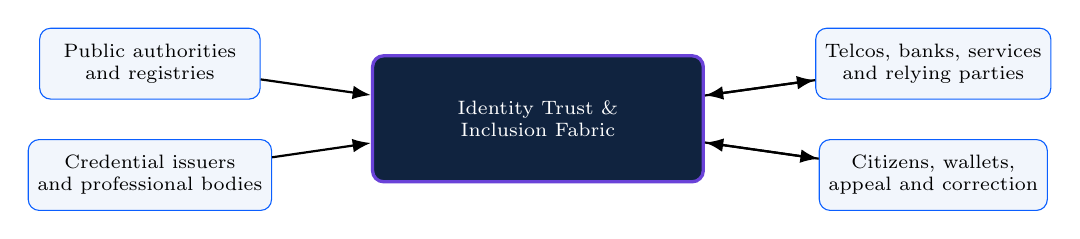
\begin{tikzpicture}[node distance=5mm and 10mm, every node/.style={font=\scriptsize}, box/.style={draw=TrustBlue,rounded corners,fill=TrustLight,minimum width=28mm,minimum height=9mm,align=center}, core/.style={draw=TrustViolet,very thick,rounded corners,fill=TrustNavy,text=white,minimum width=42mm,minimum height=16mm,align=center}]
\node[box] (gov) {Public authorities\\and registries};
\node[box,below=of gov] (issuer) {Credential issuers\\and professional bodies};
\node[core,right=14mm of gov,yshift=-7mm] (fabric) {Identity Trust \&\\Inclusion Fabric};
\node[box,right=14mm of fabric,yshift=7mm] (private) {Telcos, banks, services\\and relying parties};
\node[box,below=of private] (citizen) {Citizens, wallets,\\appeal and correction};
\draw[-{Latex},thick] (gov) -- (fabric);
\draw[-{Latex},thick] (issuer) -- (fabric);
\draw[-{Latex},thick] (private) -- (fabric);
\draw[-{Latex},thick] (citizen) -- (fabric);
\draw[-{Latex},thick] (fabric) -- (private);
\draw[-{Latex},thick] (fabric) -- (citizen);
\end{tikzpicture}
\caption{The Fabric is an assurance layer across domains, not a replacement for their authoritative systems.}
\label{fig:ecosystem}
\end{figure}

\section{Fraud and exclusion are dual system risks}

Security programmes naturally optimize the probability of admitting an attacker. Identity programmes also create the opposite harm: denying or delaying a legitimate person's access to identity, connectivity, qualification, benefits, mobility, or work. Exclusion may be produced by a poor sensor, inaccessible interface, missing alternative path, repeated document loop, obsolete record, migration conflict, over-conservative threshold, or under-resourced review process.

The engineering objective must consequently be dual:

\begin{equation}
\min_{\pi}\; \lambda_F C_F + \lambda_E C_E + \lambda_X C_X + \lambda_H C_H + \lambda_P C_P,
\label{eq:dual-objective}
\end{equation}

where $C_F$ is residual fraud cost, $C_E$ exclusion cost, $C_X$ legitimate-user friction, $C_H$ scarce human effort, and $C_P$ privacy intrusion. The action policy $\pi$ is constrained by assurance, law, purpose, review capacity, service time, and the existence of an accessible remedy.

This is not an assertion that every cost can be monetized or collapsed into one scalar. Equation~\ref{eq:dual-objective} is a decision aid. Fundamental rights, prohibited uses, minimum safeguards, and non-discrimination remain hard constraints.

\section{Research and industrial question}

The central question is:

\begin{quote}
How can a system integrator build a federated, purpose-bound identity and credential assurance capability that learns when to trust biometric and credential evidence, detects known and unknown abuse as well as systemic exclusion, requests the least additional evidence necessary, allocates scarce human expertise, and repairs the record when the system is wrong?
\end{quote}

The industrial question is distinct:

\begin{quote}
Which parts are repeatable and defensible as a product across government, telecom, regulated industry, professional credentials, and citizen wallets, and which parts must remain customer-specific policy, data, and governance?
\end{quote}

\section{Scope and exclusions}

The thesis covers score-level and structured evidence, verifiable credentials, process telemetry, graph relationships, decision policy, and remedy. It excludes the creation of a production matcher, the training of biometric recognition models on raw images, a national population database, covert surveillance, generalized AML transaction monitoring, and autonomous determination of criminal guilt. No operational deployment is implied by the demonstrator.

\chapter[Scientific, Technical, and Market Foundations]{Scientific, Technical, and Market\\Foundations}

\section{Biometric evidence and multimodal fusion}

Biometric systems transform captured physical or behavioural signals into templates and comparison scores. Their errors are characterized through false-match and false-non-match behaviour, often visualized with ROC or DET curves. Identification adds candidate-list and open-set considerations. These measurements describe matcher behaviour under a test protocol; they are not fraud metrics.

Multimodal fusion combines evidence from face, fingerprint, iris, voice, or other sources. Fusion can occur at sensor, feature, score, rank, or decision level. For industrial integration, score-level fusion is often practical because suppliers can retain proprietary templates while exposing normalized scores, quality, and provenance. Quality-dependent and cost-sensitive fusion research shows why acquiring every modality is not always optimal: sequentially requesting evidence until confidence is sufficient can improve the security--cost trade-off \citep{poh2009quality}.

The proposed Fabric generalizes sequential fusion. It treats an additional biometric, authoritative source, credential proof, or human review as an action with cost, delay, privacy, and expected information gain.

\section{Anomaly detection: modelling normality}

When confirmed anomalies are scarce and heterogeneous, a model can learn the distribution or support of nominal observations. In the density-estimation formulation, a new event is flagged when

\begin{equation}
p(x_{\mathrm{test}}\mid c)<\varepsilon_c,
\end{equation}

where $c$ is context such as channel, sensor, issuer, site, credential type, or time regime. The contextual term is essential: what is rare for a controlled office may be routine for a field enrollment station.

Isolation Forest estimates anomaly by the ease with which random partitions isolate a sample \citep{liu2008isolation}. Deep SVDD learns a representation that concentrates nominal samples around a centre \citep{ruff2018deep}. These methods are useful for novel attack or process patterns, but their semantic conclusion is limited:

\begin{equation}
\text{statistical anomaly}\not\Rightarrow\text{fraud, guilt, or invalid entitlement}.
\end{equation}

An anomaly is an investigation trigger, a request for evidence, or a signal that the model's regime assumptions require revision.

\section{Supervised learning and selective prediction}

Known fraud patterns can be learned from confirmed labels. Yet labels in identity systems are delayed, selective, and shaped by investigation capacity. A supervised model may learn past detection policy rather than underlying fraud. Weak supervision, expert scenarios, hard negatives, and counterfactual pairs can expand coverage, but generated labels must remain distinguishable from confirmed outcomes \citep{ratner2017snorkel}.

Selective prediction adds abstention. The system automates only where evidence and calibration satisfy a policy; elsewhere it requests information or human judgment. Coverage and risk among automated cases are therefore more informative than aggregate accuracy.

\section{Graph learning and relational fraud}

Fraud is frequently relational. One identity event may appear plausible, while a network of identities reusing devices, addresses, IPs, phones, documents, issuers, or operators reveals coordination. Let $G=(V,E,X)$ contain entities, relations, and node features. A graph convolutional layer can be written

\begin{equation}
H^{(l+1)}=\sigma\left(\hat{D}^{-1/2}\hat{A}\hat{D}^{-1/2}H^{(l)}W^{(l)}\right),
\end{equation}

following the normalized message-passing form popularized by \citet{kipf2017semi}. The earlier National Identity Fraud Risk Engine demonstrated, on synthetic ring-held-out data, that relational signal can outperform event-only baselines. That result establishes a research direction, not transferable field performance.

Graph evidence creates special risks. Connections may be legitimate, edges may be noisy, and highly connected infrastructure may reflect a shared office or low-income community rather than collusion. The graph must retain edge provenance, time, purpose, confidence, and alternative explanations.

\section{Verifiable credentials and federated identity}

The W3C Verifiable Credentials Data Model 2.0 formalizes an issuer--holder--verifier ecosystem and tamper-evident claims \citep{w3cvc2025}. OpenID4VCI and OpenID4VP define interoperable issuance and presentation protocols \citep{openid4vci2025,openid4vp2025}. Status lists support privacy-preserving credential status, while confidence methods can strengthen assurance that a presenter is appropriately related to the credential \citep{w3cstatus2025,w3cconfidence2026}.

Cryptography answers bounded questions: who signed, whether content changed, whether a status proof is valid, and what was disclosed. It does not guarantee that the issuer was properly accredited, that the source record was correct, that the holder-binding process was inclusive, or that a relying party requested a proportionate claim. Those are assurance and governance questions for the Fabric.

\section{Market structure}

The market is real and crowded, but segmented. Biometric vendors provide matching, PAD, liveness, and identity proofing. Behavioural-biometric platforms model sessions. Digital-identity platforms combine documents, face, liveness, trusted sources, and fraud signals. Graph-based products identify cross-transaction relationships and fraud rings. ABIS platforms address duplicate enrollment and identification.

The closest public examples include IDEMIA identity proofing, iProov active biometric threat management, Entrust/Onfido document and biometric fraud analytics, BioCatch behavioural intelligence, Mitek's layered identity platform, and Jumio 360 Fraud Analytics. Jumio publicly describes graph-database and machine-learning analysis of cross-transaction clusters \citep{jumio360}; this directly invalidates any novelty claim based solely on using graphs for identity fraud.

The proposed whitespace is the governed combination in 
\cref{tab:whitespace}.

\begin{table}[htbp]
\centering
\caption{Candidate industrial differentiation.}
\label{tab:whitespace}
\begin{tabularx}{\textwidth}{p{36mm}YY}
\toprule
Dimension & Common market emphasis & Proposed Fabric emphasis\\
\midrule
Biometrics & Face onboarding, liveness, document check & Vendor-neutral fingerprint, face, optional iris, quality, and provenance\\
Decision unit & One onboarding or authentication & Purpose-bound identity or credential assurance across lifecycle\\
Deployment & Platform or cloud service & Sovereign, on-premise, federated, restricted-domain capable\\
Learning & Known fraud or vendor threat intelligence & Known fraud + open-set anomaly + graph + process exclusion\\
Human role & Manual review queue & Selective action, operator protection, appeal, and record repair\\
Social outcome & Conversion and fraud loss & Fraud, exclusion, accessibility, delay, and remedy effectiveness\\
\bottomrule
\end{tabularx}
\end{table}

The market analysis is a July 2026 public-source snapshot, not a complete procurement evaluation. Product claims must be tested through demonstrations, technical questionnaires, customer references, independent evaluation, and legal review.

\chapter{Research Design and Contributions}

\section{Design-science position}

The work follows a design-science logic: characterize a consequential industrial problem, formulate an artifact, implement a falsifiable proof of function, evaluate it under declared limitations, and derive a controlled path to field validation. The artifact is not one algorithm. It is a socio-technical decision system comprising evidence schemas, models, policy, human roles, process telemetry, remedy, and operational governance.

The unit of success is therefore not ``model accuracy''. It is a demonstrable improvement in a governed identity decision at a controlled cost and harm level.

\section{Research questions}

\begin{description}
\item[RQ1 --- Evidence.] How can heterogeneous biometric, credential, device, graph, and process evidence be normalized without erasing source-specific uncertainty and provenance?
\item[RQ2 --- Novelty.] Does adding an anomaly detector improve the discovery of fraud patterns deliberately withheld from supervised learning at a controlled review rate?
\item[RQ3 --- Relational structure.] Does graph-derived risk add useful information beyond event-level evidence under ring-held-out and temporal splits?
\item[RQ4 --- Action.] Can a constrained policy reduce unnecessary evidence acquisition and expert work while meeting an identity-risk limit?
\item[RQ5 --- Inclusion.] Can process anomaly detection identify legitimate-user pathways with excessive attempts, delay, abandonment, or manual routing without using group membership as an adverse decision feature?
\item[RQ6 --- Remedy.] Can contestation and correction be represented as deterministic, testable state transitions whose propagation is measurable?
\item[RQ7 --- Product.] Which capabilities generalize across customers and which must remain local policy, data, and accountability?
\end{description}

\section{Hypotheses}

\begin{description}
\item[H1.] Rules plus calibrated supervised learning improve recall of confirmed suspicious inconsistencies at a fixed review capacity compared with rules alone.
\item[H2.] Anomaly detection improves recall on held-out novelty, but only when conditioned or segmented by operational regime.
\item[H3.] Relational graph evidence improves coordinated-abuse ranking over independent-event models, provided that complete rings and temporal periods are isolated across splits.
\item[H4.] A selective policy with explicit abstention reduces error among automated decisions compared with forced binary classification.
\item[H5.] Sequential evidence acquisition reduces average friction and acquisition cost while respecting a maximum residual-risk constraint.
\item[H6.] Process telemetry detects systemic exclusion patterns that security-only evaluation misses.
\item[H7.] Deterministic remedy and record-repair controls reduce the persistence of unsupported adverse states after an overturned suspicion.
\item[H8.] Component, data, model, human, and policy provenance improves diagnosis under sensor, matcher, issuer, and configuration changes.
\end{description}

\section{Claim hierarchy}

The thesis distinguishes four levels of evidence:

\begin{enumerate}
\item \textbf{Executable concept}: interfaces, dataflow, and models run end to end.
\item \textbf{Synthetic proof of function}: controlled planted patterns are detected under leakage-resistant splits.
\item \textbf{Retrospective field evidence}: historical operational data show calibrated usefulness without production action.
\item \textbf{Prospective operational evidence}: shadow and controlled-support pilots demonstrate stable value, non-exclusion, and remedy under real workflows.
\end{enumerate}

This package reaches levels 1 and 2 only. Product claims require levels 3 and 4.

\section{Contributions}

\subsection{Conceptual contributions}

The first contribution is the dual-risk formulation in which fraud and exclusion are co-equal system failures. The second is the distinction among evidence, anomaly, suspicion, confirmed fraud, administrative error, and adverse action. The third is a federated evidence-graph concept that connects issuers, credentials, holder binding, verifiers, devices, processes, and remedies without requiring a universal citizen graph.

\subsection{Technical contributions}

The technical artifact combines:

\begin{itemize}
\item a versioned evidence envelope;
\item supervised known-fraud prediction;
\item open-set anomaly scoring;
\item graph-derived relational risk;
\item process-exclusion anomaly scoring;
\item calibrated fusion and action bands;
\item a deterministic remedy state machine;
\item synthetic generation, temporal holdout, and reproducible evaluation.
\end{itemize}

\subsection{Industrial contributions}

The industrial artifact provides a product boundary, market whitespace, build--buy--partner decision, requirements canvas, deployment stages, roles, metrics, and investment gates. It deliberately prevents the research thesis from becoming an unbounded platform claim.

\section{Evaluation matrix}

\begin{table}[htbp]
\centering
\caption{Evaluation levels and representative questions.}
\begin{tabularx}{\textwidth}{p{31mm}YY}
\toprule
Level & Technical question & Operational question\\
\midrule
Signal & Does the score separate planted outcomes? & Is the signal available, lawful, stable, and interpretable?\\
Fusion & Does combination add value in ablation? & Does it reduce residual risk at fixed burden?\\
Policy & Are actions consistent with thresholds and constraints? & Is the chosen evidence or review proportionate?\\
Lifecycle & Does drift or version change degrade calibration? & Can the system roll back and explain decisions?\\
Remedy & Does correction update all dependent states? & Can a person obtain accessible, timely redress?\\
Ecosystem & Do federated proofs interoperate? & Are authority, liability, and purpose clear across organizations?\\
\bottomrule
\end{tabularx}
\end{table}

\section{Epistemic cautions}

Five confusions are explicitly prohibited:

\begin{align}
\text{cluster} &\neq \text{real causal regime},\\
\text{anomaly} &\neq \text{fraud},\\
\text{graph proximity} &\neq \text{complicity},\\
\text{valid signature} &\neq \text{true underlying claim},\\
\text{human review} &\neq \text{absence of automation bias}.
\end{align}

Labels are generated by socio-technical processes. Investigation effort changes which fraud becomes visible. False suspicion may persist in records and later be treated as ground truth. Evaluation must therefore track label source, certainty, contestation, and repair state.

\chapter{Federated Product Architecture}

\section{Architectural principles}

The architecture is governed by nine principles:

\begin{enumerate}
\item \textbf{Purpose before data}: every query is tied to a declared service and authorized decision.
\item \textbf{Minimum necessary proof}: request a derived claim or proof rather than a full source record when possible.
\item \textbf{Authoritative data remain authoritative}: the Fabric does not silently become a shadow registry.
\item \textbf{No universal person score}: assessments are transaction-, credential-, and purpose-specific.
\item \textbf{Evidence is versioned}: source, time, quality, policy, and model provenance are inseparable from a score.
\item \textbf{Anomaly is a hypothesis}: it triggers investigation or step-up, not guilt.
\item \textbf{Inclusion is observable}: delay, repetition, abandonment, alternative paths, and remedies are instrumented.
\item \textbf{Humans are governed components}: roles, evidence views, workload, overrides, and protection are designed and evaluated.
\item \textbf{Correction propagates}: an overturned decision must repair dependent states and verify completion.
\end{enumerate}

\section{Layered view}

\begin{figure}[H]
\centering
\resizebox{\textwidth}{!}{%
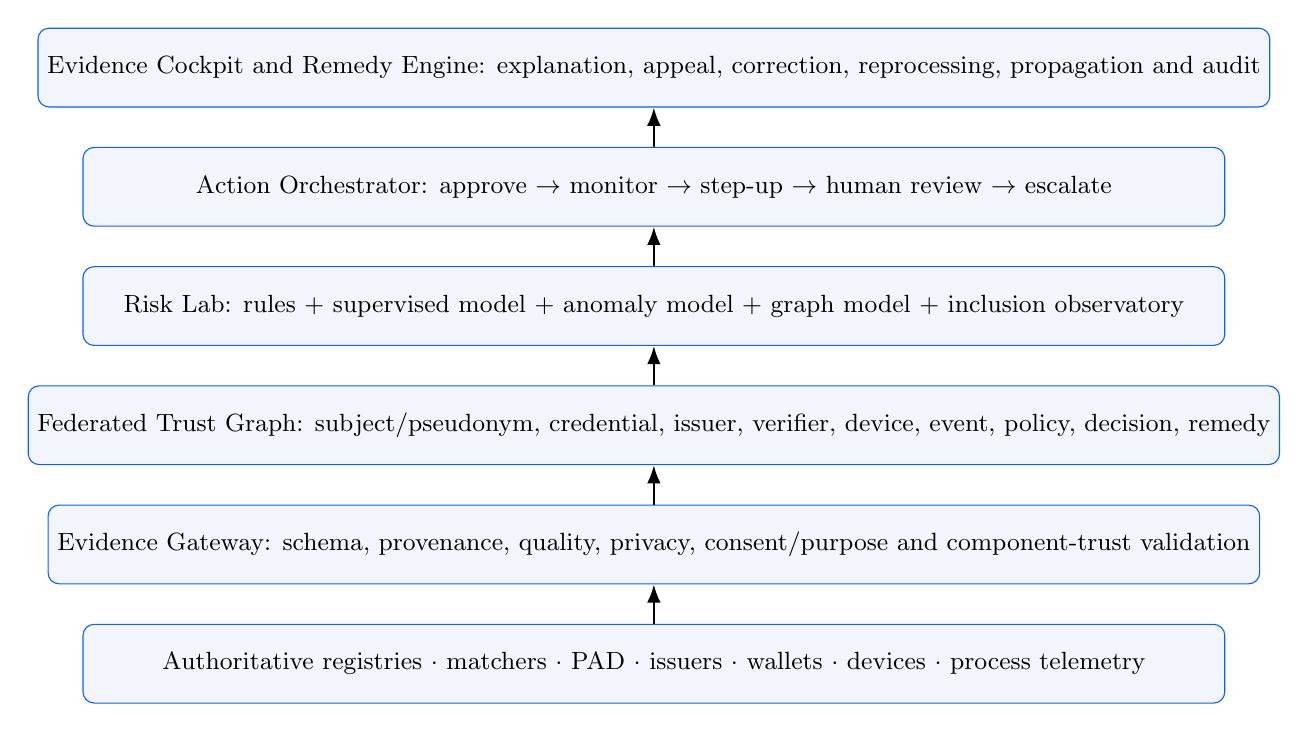
\begin{tikzpicture}[node distance=5mm, every node/.style={font=\small}, layer/.style={draw=TrustBlue,rounded corners,fill=TrustLight,minimum width=145mm,minimum height=10mm,align=center}]
\node[layer] (sources) {Authoritative registries $\cdot$ matchers $\cdot$ PAD $\cdot$ issuers $\cdot$ wallets $\cdot$ devices $\cdot$ process telemetry};
\node[layer,above=of sources] (gateway) {Evidence Gateway: schema, provenance, quality, privacy, consent/purpose and component-trust validation};
\node[layer,above=of gateway] (graph) {Federated Trust Graph: subject/pseudonym, credential, issuer, verifier, device, event, policy, decision, remedy};
\node[layer,above=of graph] (analytics) {Risk Lab: rules $+$ supervised model $+$ anomaly model $+$ graph model $+$ inclusion observatory};
\node[layer,above=of analytics] (policy) {Action Orchestrator: approve $\rightarrow$ monitor $\rightarrow$ step-up $\rightarrow$ human review $\rightarrow$ escalate};
\node[layer,above=of policy] (remedy) {Evidence Cockpit and Remedy Engine: explanation, appeal, correction, reprocessing, propagation and audit};
\draw[-{Latex},thick] (sources) -- (gateway);
\draw[-{Latex},thick] (gateway) -- (graph);
\draw[-{Latex},thick] (graph) -- (analytics);
\draw[-{Latex},thick] (analytics) -- (policy);
\draw[-{Latex},thick] (policy) -- (remedy);
\end{tikzpicture}
}
\caption{Reference architecture. Each layer has independent evidence and assurance obligations.}
\label{fig:architecture}
\end{figure}

\section{Evidence envelope}

Every observation is carried in an envelope rather than as an anonymous scalar:

\begin{equation}
e=\langle id,type,value,quality,source,time,context,purpose,version,confidence,access\rangle.
\end{equation}

For a fingerprint matcher score, the envelope includes matcher and model version, sensor, finger positions, aggregation method, image-quality measures, threshold policy, missing-finger semantics, and whether the value was obtained from a Matcher Mock or a real matcher. For a credential, it includes issuer identifier, schema, proof format, issuance and expiry, status method, accreditation reference, disclosed claims, holder-binding method, and verifier request purpose.

This prevents a common failure: interpreting the same numeric score as equivalent across suppliers, versions, contexts, or populations.

\section{Trust graph ontology}

The graph is heterogeneous and temporal. Candidate node types include subject pseudonyms, credentials, issuers, verifiers, wallets, devices, services, processes, evidence bundles, policies, decisions, reviews, and remedies. Edge types include \emph{issued-by}, \emph{presented-by}, \emph{verified-at}, \emph{bound-to}, \emph{derived-from}, \emph{reviewed-by}, \emph{overturned-by}, and \emph{repaired-at}.

Every edge has time, source, purpose, confidence, and retention metadata. Cross-domain linkage uses scoped pseudonyms or privacy-preserving matching. The design rejects a permanent global key joining all citizen activity.

\section{Action orchestration}

Let $b$ denote available evidence and $a$ a candidate action. A decision policy selects

\begin{equation}
\pi(b)=\arg\min_{a\in\mathcal{A}}\; \mathbb{E}[C(a,Y)\mid b]
\end{equation}

subject to mandatory controls. The action set can be

\begin{equation}
\begin{split}
\mathcal{A}=\{&approve,monitor,request\_finger,request\_face,\\
              &verify\_credential,human\_review,escalate\}.
\end{split}
\end{equation}

The policy can request evidence expected to reduce uncertainty most per unit cost. It must also allow ``cannot decide'' and ``alternative accessible path'' states. A block or administrative adverse action is never derived merely from a novelty score.

\section{Remedy and record repair}

Earlier \emph{Beyond the Matcher} work introduced CETRA-R: capture, evaluate, treat, review, appeal, and repair. The Fabric turns remedy into an executable state machine:

\begin{equation}
\begin{aligned}
s_0=suspected&\rightarrow s_1=reviewed\\
&\rightarrow
\begin{cases}
s_2=confirmed,\\
s_3=overturned\rightarrow s_4=repaired\\
\hspace{22mm}\rightarrow s_5=propagation\_verified.
\end{cases}
\end{aligned}
\end{equation}

Repair is not deletion of audit history. It is preservation of the original evidence and decision while ensuring that unsupported adverse labels no longer drive future decisions. The system records affected relying parties, reprocessing policy, notification basis, completion, and residual exceptions.

\section{Deployment topology}

The architecture supports three domains:

\begin{itemize}
\item \textbf{Open}: public schemas, trust lists, non-sensitive standards, and published model documentation;
\item \textbf{Sovereign}: government or regulated-customer evidence and models, on-premise or controlled cloud;
\item \textbf{Restricted}: raw biometrics, investigative data, secret linkage, cryptographic keys, and legally constrained intelligence.
\end{itemize}

Only approved derived signals cross boundaries. Model training can be local, federated, or based on synthetic scenarios. Observability transports pseudonymous trace identifiers and metric aggregates, never reusable biometric payloads.

\section{Integration with existing systems}

The Fabric integrates rather than replaces:

\begin{itemize}
\item ABIS and matchers for biometric comparison;
\item PAD and injection detectors for capture assurance;
\item document and credential validators;
\item wallets and OpenID4VC protocols;
\item registries and trust lists;
\item case-management and investigation systems;
\item OpenTelemetry-compatible observability and evidence stores;
\item DMN or policy-as-code decision services.
\end{itemize}

The first interface contract should be implemented before any ML model: it is the stable product seam across suppliers and customer-specific policies.

\chapter{Hybrid Models and Constrained Decision Policy}

\section{Feature families}

For an event $i$, the research vector is partitioned by meaning and governance:

\begin{equation}
x_i=[x_i^{bio},x_i^{cred},x_i^{device},x_i^{beh},x_i^{graph},x_i^{process},x_i^{prov}].
\end{equation}

Biometric evidence includes face, fingerprint, optional iris scores, per-modality quality, failure-to-acquire, and PAD. Credential evidence includes signature, issuer trust, status, schema, expiry, accreditation, and holder-binding confidence. Device and behaviour include integrity, reuse, velocity, and session indicators. Graph features summarize scoped relational structure. Process features include attempts, duration, abandonment, manual routing, alternative path, and remedy state. Provenance features describe versions and component trust.

Protected or sensitive attributes are not automatically model features. They may be required for controlled fairness evaluation, but their availability, separation, purpose, and access require explicit governance.

\section{Known-fraud model}

The supervised model estimates

\begin{equation}
\hat{p}_S(x)=P(Y=fraud\mid x,D_L),
\end{equation}

where $D_L$ contains labelled cases with source and certainty. Suitable interpretable baselines include logistic regression and constrained decision trees. Random forests or gradient boosting can model nonlinear interactions, while calibration maps model scores to decision-useful probabilities.

Evaluation uses temporal or project separation rather than random event splitting alone. All events from a fraud ring, credential campaign, device family, or issuer incident must remain in one partition where the claim concerns generalization.

\section{Novelty model}

The novelty component is trained primarily on nominal data:

\begin{equation}
a(x,c)=-\log \hat{p}(x\mid c)
\end{equation}

or, for Isolation Forest, on normalized isolation score. Context $c$ prevents a minority operational regime from being labelled anomalous merely because it is less frequent. Candidate contexts include channel, site, sensor family, credential type, issuer category, and time regime.

Novelty must expose contributing deviations: for example, high face match paired with implausibly low quality, active credential paired with invalid issuer accreditation, or high process burden for a legitimate low-risk journey.

\section{Graph risk}

The graph model estimates $\hat{p}_G(v,G_t)$ from topology, temporal edges, and permitted features. Baselines are required before a GNN:

\begin{itemize}
\item degree and shared-attribute counts;
\item rule score for impossible or excessive reuse;
\item logistic regression or MLP on engineered graph features;
\item GCN, GraphSAGE, or heterogeneous GNN.
\end{itemize}

A GNN is justified only if it outperforms strong structural baselines under ring-held-out and time-held-out evaluation, retains calibrated utility, and provides investigator-usable explanations. Edge ablations test whether the model relies on a defensible relation rather than leakage.

\section{Inclusion-risk model}

The inclusion model is deliberately separate from fraud inference. Among legitimate or subsequently cleared journeys, it estimates the probability of excessive burden:

\begin{equation}
q_E=P(\text{repeat, delay, abandonment, inaccessible path, or unresolved remedy}\mid c).
\end{equation}

An unsupervised version compares process duration, attempts, capture failures, and manual routing with context-specific baselines. A supervised version can learn from confirmed process failures and complaints. Aggregated monitoring identifies site, device, issuer, channel, language, accessibility, and temporal patterns where lawful and proportionate.

The output is a process-improvement or support signal. It must not be used to reduce a person's entitlement or increase suspicion because that person encountered difficulty.

\section{Fusion}

A simple research fusion is

\begin{equation}
r=w_S\tilde{p}_S+w_A\tilde{a}+w_G\tilde{p}_G+w_R r_{rules},
\end{equation}

where each component is normalized and calibrated on validation data. More advanced alternatives include stacking, Bayesian networks, mixture-of-experts, or evidential reasoning. Missing modalities require explicit treatment; zero must not silently mean missing.

Uncertainty is represented separately from risk. Low risk with high uncertainty may require more evidence. High risk with well-understood evidence may require a policy-specific review. The decision surface is therefore two-dimensional or higher:

\begin{equation}
a=\pi(r,u,q_E,c,capacity).
\end{equation}

\section{Action bands}

The baseline policy uses bands:

\begin{table}[htbp]
\centering
\caption{Illustrative action bands; values are not production thresholds.}
\begin{tabularx}{\textwidth}{p{28mm}p{28mm}Y}
\toprule
Risk band & Default action & Required control\\
\midrule
$r<0.35$ & Approve & retain evidence provenance and monitor drift\\
$0.35\le r<0.55$ & Monitor & no extra citizen burden unless another control requires it\\
$0.55\le r<0.72$ & Step-up & select least intrusive evidence expected to reduce uncertainty\\
$0.72\le r<0.90$ & Human review & show evidence, alternatives, limitations, and policy version\\
$r\ge0.90$ & Block or escalate candidate & require rule-authorized corroboration; anomaly alone is insufficient\\
\bottomrule
\end{tabularx}
\end{table}

Thresholds are chosen under review-capacity and cost constraints, never copied from the synthetic demonstrator.

\section{Metrics}

The metric suite separates layers:

\begin{itemize}
\item matcher: FMR/FNMR, FPIR/FNIR, TMR at target FMR, ROC/DET, failure to acquire;
\item fraud ranking: ROC AUC, average precision, recall at 5/10/20\% review, precision in the review queue;
\item novelty: held-out attack recall, time-to-detection, false-alert rate by regime;
\item calibration: Brier score, reliability curve, expected calibration error;
\item action: automation coverage, selective risk, evidence cost, human hours, latency;
\item inclusion: completion, attempts, delay, abandonment, alternative-path success, unresolved remedy;
\item lifecycle: drift, version sensitivity, rollback success, evidence and correction propagation.
\end{itemize}

Accuracy is not a primary metric under rare fraud because an always-normal model can appear accurate while being useless.


\chapter{Synthetic Proof of Function}

\section{Purpose and claim boundary}

The experiment verifies that the proposed pipeline is executable, that withheld novelty can be evaluated, that relational reuse contributes a separate signal, and that inclusion monitoring can identify planted process burdens. It is intentionally small and transparent. It does not simulate a country's population, a vendor matcher, human behaviour, or real fraud economics.

\claimboundary

\section{Generator}

The controlled generator creates 12,000 events across 24 synthetic months, 6,500 identities, 1,800 devices, 45 issuers, four channels, and five credential types. Each event contains score-level face and fingerprint evidence, optional iris, quality, liveness, document score, issuer trust, credential status, device risk, velocity, process attempts, duration, and labels known only to the experiment.

Fraud is planted in two families:

\begin{enumerate}
\item \textbf{Known patterns} with degraded matcher/document/liveness evidence, risky devices, and high velocity. These examples are available to supervised training.
\item \textbf{Novel coherence patterns} with plausible fingerprint, liveness, and document scores but an unusual cross-modal combination, including low face compatibility. These examples are excluded from supervised training labels and are intended to test anomaly and graph contribution.
\end{enumerate}

Fraud events reuse a limited device pool to produce relational signal. Legitimate exclusion cases receive additional attempts, longer duration, and quality burden, particularly in a planted kiosk and late partner-channel regime. These process cases must never increase fraud risk merely because the citizen struggled.

\section{Temporal split and leakage controls}

The final 25\% of the time horizon is held out. Preprocessing and models are fit on the earlier period. Novel fraud is withheld from the supervised label set. Device-reuse counts are computed from training evidence only. No target label is used as an input feature.

This split is still weaker than a full industrial evaluation. A future protocol will separate complete rings, issuers, sites, projects, credential campaigns, and model versions, and will include a composition holdout combining known factors in unseen ways.

\section{Models}

The demonstration uses:

\begin{itemize}
\item a class-weighted random forest for known-fraud patterns;
\item Isolation Forest trained on nominal evidence;
\item a device-reuse and device-risk relational baseline;
\item robust channel-conditioned duration and attempt scoring for exclusion;
\item fixed weighted fusion $w_S=0.50$, $w_A=0.25$, $w_G=0.25$.
\end{itemize}

The relational component is deliberately not called a GNN. It is a baseline that tests the graph hypothesis before model complexity. The separate GNN repository remains the appropriate experimental line for full message passing and ring-held-out comparisons.

\section{Results}

The temporal test set contains \TestN{} events at a fraud prevalence of \FraudRate{}. The hybrid score obtains ROC AUC \RocAuc{}, average precision \AvgPrecision{}, and Brier score \Brier{}. At a top-\ReviewCapacity{} review capacity, fraud recall is \RecallCapacity{} and recall on deliberately withheld novel fraud is \NovelRecall{}. The process-exclusion score obtains ROC AUC \ExclusionAuc{} against planted exclusion labels.

\begin{figure}[htbp]
\centering
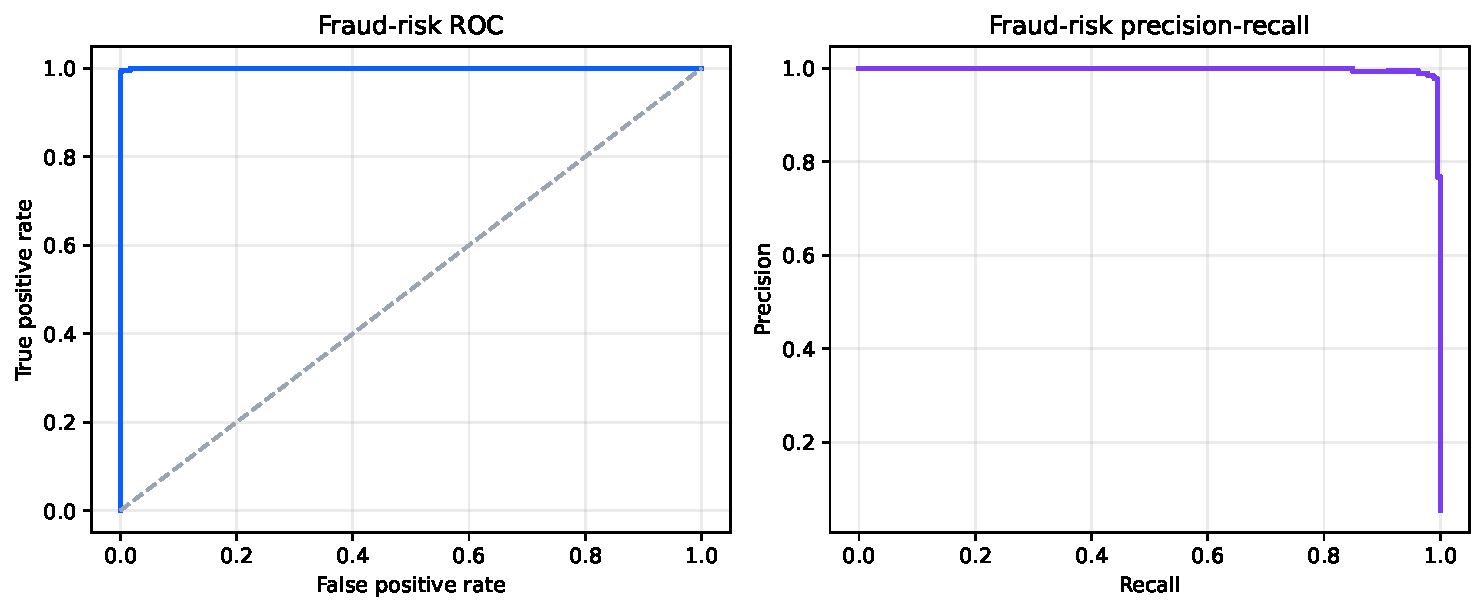
\includegraphics[width=0.92\textwidth]{../figures/fraud_curves.pdf}
\caption{Synthetic fraud-ranking curves. These are pipeline checks, not operational product claims.}
\label{fig:fraud-curves}
\end{figure}

\begin{figure}[htbp]
\centering
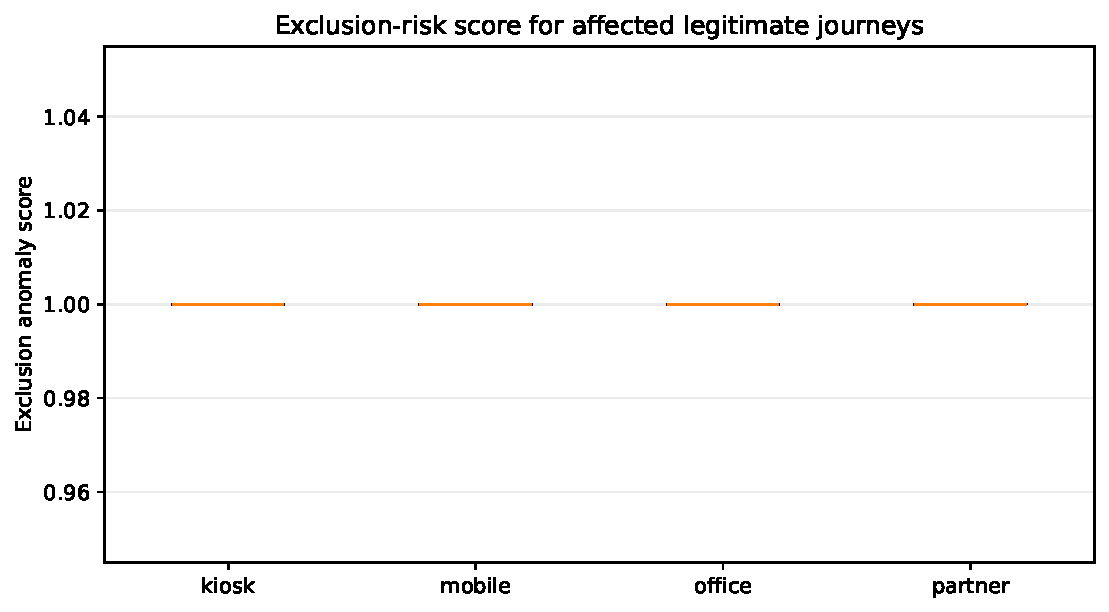
\includegraphics[width=0.78\textwidth]{../figures/exclusion_by_channel.pdf}
\caption{Synthetic exclusion scores for planted affected legitimate journeys by channel.}
\label{fig:exclusion}
\end{figure}

The expected interpretation is limited. High performance is partly a property of the planted generator. It confirms that the code, split, score fusion, metrics, and paper-generation chain are coherent. It does not validate feature realism, attacker adaptation, fairness, calibration transfer, legal admissibility, or field utility.

\section{Required ablations}

A publishable empirical programme must compare:

\begin{enumerate}
\item rules only;
\item logistic regression and tree baselines;
\item supervised model only;
\item anomaly model only;
\item relational structural baseline;
\item GNN with ring-held-out split;
\item supervised + anomaly;
\item supervised + graph;
\item full hybrid;
\item full hybrid with action policy and inclusion observatory.
\end{enumerate}

Additional ablations remove modality quality, component provenance, graph edge types, regime conditioning, remedy features, and synthetic hard negatives. A permuted graph and permuted regime assignment test whether improvements depend on meaningful structure.

\section{Field-validation protocol}

Field validation proceeds in five gates:

\begin{description}
\item[Gate 0 --- Contract.] Agree purpose, outcomes, ground-truth states, evidence, retention, actions, review, and remedy.
\item[Gate 1 --- Retrospective.] Replay historical events without changing decisions; measure leakage, calibration, segments, and label quality.
\item[Gate 2 --- Shadow.] Run prospectively with no user or operator impact; compare current and proposed decisions.
\item[Gate 3 --- Controlled support.] Rank a bounded expert queue and recommend evidence gaps; the authorized process retains final control.
\item[Gate 4 --- Governed production.] Automate only approved low-risk actions, with rollback, monitoring, appeal, and independent assurance.
\end{description}

The study must pre-register primary metrics and stopping conditions. A system may be technically predictive and still receive REDESIGN or NO-GO because purpose, proportionality, inclusion, explainability, or remedy is inadequate.

\section{Threats to validity}

\begin{itemize}
\item \textbf{Synthetic realism}: planted patterns may be easier than real fraud.
\item \textbf{Selection bias}: confirmed fraud overrepresents cases that current systems can already detect.
\item \textbf{Investigation bias}: review capacity shapes the labels used for training.
\item \textbf{Temporal adaptation}: attackers respond to deployed controls.
\item \textbf{Context shift}: sites, devices, issuers, and policies change.
\item \textbf{Graph error}: shared infrastructure can be legitimate and edges may be stale.
\item \textbf{Outcome ambiguity}: anomaly, administrative error, attempted fraud, and confirmed fraud require separate states.
\item \textbf{Fairness measurement}: aggregate parity can hide individual and intersectional harm.
\item \textbf{Automation bias}: human review can amplify rather than correct a model signal.
\end{itemize}


\chapter{Governance, Rights, Security, and Assurance}

\section{A trust platform must not become a surveillance platform}

The internal analogy of a ``Palantir for identity'' describes ontology, evidence fusion, relational investigation, and traceability. It is unsafe as an unconstrained product doctrine. A centralized graph of citizen activity, permanent cross-domain identifiers, opaque suspicion scores, or unrestricted secondary use would contradict the stated mission.

The external doctrine is therefore \emph{federated assurance}: authoritative sources retain their records, proofs are purpose-limited, linkage is scoped, and citizens can understand and challenge consequential outcomes.

\section{Purpose and proportionality gate}

Before integration or model development, a cross-functional authority records:

\begin{itemize}
\item legitimate purpose and protected decision;
\item necessity of identity, credential, and biometric evidence;
\item less intrusive alternatives;
\item affected persons, including those not considered direct users;
\item plausible harms, misuse, and purpose drift;
\item legal basis, retention, access, and cross-domain sharing;
\item alternative path, contestation, remedy, and accountability;
\item GO, GO WITH RESTRICTIONS, PILOT, REDESIGN, or NO-GO outcome.
\end{itemize}

NIST SP 800-63A-4 requires a documented fraud-management programme and privacy-risk assessment for fraud controls \citep{nist63a4}. NIST federation guidance also emphasizes accessible redress \citep{nist63c4}. These controls are not compliance decorations; they are system requirements.

\section{Privacy architecture}

The data-minimization hierarchy is:

\begin{enumerate}
\item cryptographic or authoritative yes/no proof;
\item selectively disclosed attribute;
\item derived and purpose-scoped risk feature;
\item pseudonymous event;
\item source record only where necessary and authorized;
\item raw or reusable biometric material only inside its dedicated protected subsystem.
\end{enumerate}

Biometric samples and templates are prohibited from general logs, traces, analytics lakes, model prompts, and graph exports. Telemetry contains pseudonymous correlation identifiers, model and policy versions, reason codes, latency, and evidence availability.

\section{Security and abuse cases}

The platform must defend against external attack and institutional misuse:

\begin{itemize}
\item forged or replayed credentials and status responses;
\item presentation, injection, deepfake, and sensor bypass;
\item compromised issuer, verifier, device, operator, or model supply chain;
\item graph poisoning, fabricated edges, and coordinated low-and-slow abuse;
\item model extraction, evasion, and inference about protected records;
\item insider browsing and unauthorized cross-domain linkage;
\item policy manipulation and threshold drift;
\item suppression of corrections or incomplete downstream repair;
\item use of inclusion telemetry to penalize people who encountered barriers.
\end{itemize}

Security controls include signed evidence bundles, mutual authentication, hardware-backed key protection where appropriate, least privilege, purpose-bound authorization, tamper-evident audit, separation of duties, rate limiting, privacy-preserving analytics, supply-chain inventories, and tested incident response.

\section{Human review and operator protection}

Human review is not a universal remedy. Reviewers can suffer automation bias, time pressure, incomplete evidence, hindsight bias, or organizational incentives. The cockpit must show:

\begin{itemize}
\item evidence source and quality;
\item what is missing;
\item model confidence and calibration limits;
\item rule and policy reasons;
\item alternative benign explanations;
\item similar cleared and confirmed cases where lawful;
\item allowed actions and escalation path;
\item an explicit option to disagree or mark insufficient evidence.
\end{itemize}

Operator actions are attributed accurately, but the system must not convert reasonable use of an approved procedure into personal blame. Provenance separates model recommendation, policy constraint, evidence availability, operator decision, and supervisory approval.

\section{Fairness and inclusion assurance}

Fairness is evaluated across the full pipeline: acquisition, quality, PAD, matching, fusion, credential verification, action, waiting time, reviewer decision, remedy, and downstream propagation. Relevant indicators include failure to acquire, false non-match, repeated evidence requests, manual-review rate, completion, delay, abandonment, appeal, overturn, and repair time.

Segment analysis must be lawful and privacy-protective. It should diagnose systems rather than create new adverse features. A difference is investigated through sensor, site, channel, process, and data mechanisms. Pure aggregate parity is insufficient; individual cases and intersectional patterns require review.

\section{Assurance case}

The production decision is supported by a structured assurance case:

\begin{description}
\item[Claim.] The Fabric supports the declared identity or credential decision with acceptable residual fraud and exclusion risk.
\item[Argument.] Evidence sources are fit for purpose; models are validated; actions are proportionate; monitoring detects drift; remedy is accessible and effective.
\item[Evidence.] Requirements, threat model, data card, model card, test results, calibration, segment analysis, operational rehearsal, incident and rollback tests, accessibility assessment, and independent review.
\end{description}

Evidence is versioned. A change in matcher, sensor, issuer trust list, credential format, model, feature pipeline, threshold, or review policy can invalidate part of the assurance case and trigger targeted re-evaluation.

\section{Accountability model}

\begin{table}[htbp]
\centering
\caption{Minimum accountability roles.}
\begin{tabularx}{\textwidth}{p{36mm}Y}
\toprule
Role & Primary accountability\\
\midrule
Purpose owner & necessity, proportionality, service outcome, and stop decision\\
Identity/biometric authority & matcher interpretation, quality, thresholds, and operational semantics\\
Fraud authority & threat ontology, investigation state, label quality, and feedback\\
Inclusion/accessibility authority & barriers, alternative path, process redesign, and outcome monitoring\\
Data protection/legal & lawful basis, minimization, sharing, retention, rights, and impact assessment\\
Model owner & data, features, validation, calibration, monitoring, and rollback\\
Decision-policy owner & action bands, human authority, review capacity, and exceptions\\
Remedy owner & appeal, correction, reprocessing, and propagation completion\\
Independent assurance & challenge of claims, evidence, conflicts, and residual risk\\
\bottomrule
\end{tabularx}
\end{table}


\chapter{Industrial and Product Opportunity}

\section{Product thesis}

The product is not another matcher, liveness SDK, KYC workflow, or generic fraud classifier. Those markets contain mature competitors. The product is a vendor-neutral assurance and action layer for organizations that already possess heterogeneous identity capabilities but lack a coherent evidence, risk, inclusion, and remedy system.

The positioning statement is:

\begin{quote}
A federated identity and credential assurance infrastructure that detects known fraud, unknown anomalies, relational abuse, systemic exclusion, and process failure while preserving privacy, human agency, and the right to redress.
\end{quote}

\section{Customer segments and jobs}

\begin{table}[htbp]
\centering
\caption{Priority customer segments and jobs to be done.}
\begin{tabularx}{\textwidth}{p{35mm}YY}
\toprule
Segment & Job & Candidate beachhead\\
\midrule
National identity authority & assure enrollment, deduplication, correction, and service access & post-matcher evidence and exclusion observatory\\
Credential ecosystem & verify issuer, status, holder binding, and accreditation & diploma/professional credential assurance\\
Telco & assure SIM onboarding, replacement, recovery, and shared-device abuse & identity--credential--device graph and step-up policy\\
Bank/regulated service & combine existing KYC, biometric, device, and behavioural signals & sovereign orchestration and review-capacity optimization\\
Enterprise/critical access & verify employee, contractor, qualification, and authorization & reusable credential and assurance policy\\
Public digital service & reduce fraud without excluding legitimate users & inclusion observatory and alternative-path orchestration\\
\bottomrule
\end{tabularx}
\end{table}

\section{Build, buy, and partner boundary}

Build the evidence ontology, normalization, provenance, customer-specific calibration, anomaly and graph fusion, inclusion observatory, action policy, remedy engine, and assurance cockpit. Buy or partner for biometric matching, PAD, document authenticity, device intelligence, sanctions/AML screening, wallet components, and general case management unless a strategic reason justifies vertical integration.

This boundary concentrates intellectual property on the decision and governance problem while preserving supplier choice.

\section{Product modules}

\begin{description}
\item[Evidence Gateway.] APIs, schemas, provenance, quality, trust-domain policy, and source adapters.
\item[Trust Graph.] Scoped identity, credential, issuer, verifier, device, process, and remedy relations.
\item[Risk Lab.] Scenario generation, truth matrix, rules, supervised models, anomaly detection, GNN experiments, calibration, and ablation.
\item[Inclusion Observatory.] Journey burden, repeated failures, delay, abandonment, alternative-path success, and systemic-pattern alerts.
\item[Action Orchestrator.] Evidence acquisition, review routing, abstention, and policy-as-code.
\item[Remedy Engine.] Appeal, correction, reprocessing, and propagation verification.
\item[Assurance Cockpit.] Role-specific investigator, operator, citizen, auditor, model-owner, and executive views.
\end{description}

\section{Commercial model}

Potential revenue layers are:

\begin{itemize}
\item annual platform license for sovereign or regulated deployment;
\item integration packs for ABIS, matchers, wallets, registries, telcos, and credential issuers;
\item per-transaction assurance API where cloud delivery is permitted;
\item calibration, monitoring, and threat-pattern subscription;
\item independent benchmark, simulation, and assurance service;
\item managed model and policy lifecycle support.
\end{itemize}

Pricing must reflect value and operating responsibility, not only transaction volume. A customer that retains decision authority, infrastructure, and investigation differs materially from a managed service in which the supplier operates models or analysts.

\section{Value model}

The business case combines avoided loss and operational improvement:

\begin{equation}
V=\Delta L_F+\Delta C_H+\Delta C_X+\Delta C_E+\Delta C_I-C_{platform},
\end{equation}

where $\Delta L_F$ is avoided fraud loss, $\Delta C_H$ expert capacity saved, $\Delta C_X$ friction reduction, $\Delta C_E$ exclusion and remediation cost reduction, and $\Delta C_I$ avoided integration and incident cost. Values must be customer-derived; the thesis provides no invented market-size or return-on-investment number.

Non-financial value includes sovereign control, audit evidence, reduced dependency on one matcher vendor, faster introduction of new credentials, and a defensible rights and accessibility posture.

\section{Competitive moat}

A model alone is not a moat. Sustainable differentiation would come from:

\begin{itemize}
\item a robust cross-vendor evidence ontology and integration library;
\item high-quality scenario, hard-negative, and counterfactual assets;
\item calibrated customer-specific decision and inclusion benchmarks;
\item privacy-preserving federated graph methods;
\item remedy and propagation controls embedded in workflow;
\item trusted deployment in sovereign and restricted environments;
\item operational knowledge connecting biometrics, identity, credentials, fraud, QA, and human review.
\end{itemize}

Data-network effects must not depend on unrestricted pooling of citizen information. Safer learning assets include de-identified patterns, federated aggregates, synthetic scenarios, red-team playbooks, model evaluation methods, and portable evidence schemas.

\section{Product risks}

The largest risks are not purely technical:

\begin{itemize}
\item product scope expands into an unmanageable universal platform;
\item a customer expects a magic fraud score without labels or investigation capacity;
\item legal and political concerns arise from graph language or centralization;
\item component vendors limit score semantics or interoperability;
\item long government sales cycles precede repeatable product fit;
\item false alerts overwhelm review and damage citizen trust;
\item inclusion monitoring is promised but not connected to process authority;
\item security and liability obligations exceed the proposed operating model.
\end{itemize}

The mitigation is a narrow beachhead, explicit non-claims, customer discovery, shadow evidence, modular integration, and a staged investment gate.

\section{Investment decision framework}

Proceed from research to product discovery when at least three conditions hold: multiple customers express the same unfilled job; lawful event and outcome data can be obtained; and a bounded pilot can measure value without adverse automation. Proceed to productization only when integration patterns repeat, calibration remains customer-manageable, and the commercial model covers support, assurance, security, and remedy obligations.

The opportunity is credible, but novelty must be stated accurately. The invention is not ``ML for fraud'' or ``graphs for identity''. It is the integrated, sovereign, rights-preserving decision fabric and its operational method.


\chapter{Industrialization Roadmap}

\section{Stage 0: turn the box into a contract}

The first deliverable for the current project is not software. It is a signed Fraud, Trust, and Inclusion Capability Contract defining purpose, scope, ontology, signals, decisions, ground truth, review, service levels, privacy, remedy, and acceptance criteria.

During a four- to six-week discovery, the team conducts threat workshops, maps current evidence, interviews fraud investigators and operators, observes legitimate-user failure journeys, inventories interfaces and versions, and evaluates candidate suppliers. The outcome is a build--buy--partner recommendation and a bounded pilot statement.

\section{Stage 1: evidence observatory}

The first technical release is read-only and non-adverse. It ingests versioned score-level evidence and process telemetry, reconstructs decision traces, and provides dashboards for:

\begin{itemize}
\item signal completeness and quality;
\item current rule outcomes;
\item review load and delay;
\item repeated legitimate-user failures;
\item policy and component-version changes;
\item missing or inconsistent evidence.
\end{itemize}

This stage creates immediate quality and governance value even if ML does not proceed.

\section{Stage 2: shadow risk lab}

Rules, supervised baselines, anomaly detection, and graph baselines run in parallel with the existing process. No production action consumes their result. The team measures disagreement, false alerts, novelty, calibration, segment stability, review-capacity curves, and process exclusion.

Shadow mode includes an explicit model-risk register, evidence gap review, and red-team scenarios. A model that merely reproduces current rules is not necessarily useless: it may reveal where the claimed innovation does not exist.

\section{Stage 3: controlled support}

The Fabric ranks a bounded queue and recommends the least additional evidence required. Authorized experts retain the decision. Interfaces collect structured feedback: confirmed fraud, cleared suspicion, insufficient evidence, administrative error, process failure, and alternative explanation.

The pilot evaluates human factors: time per case, confidence, disagreement, automation bias, reason usefulness, operator stress, and quality of record repair.

\section{Stage 4: federated credential and graph pilot}

A second organization or credential domain is added. Candidate pilots include diploma or professional credential assurance, telco SIM replacement, or cross-channel identity recovery. OpenID4VC issuance/presentation, credential status, issuer trust, scoped pseudonyms, and graph features are tested without creating a central activity lake.

Interoperability and governance are success criteria equal to model performance.

\section{Stage 5: governed production}

Only low-risk, approved actions are automated initially. Production requires:

\begin{itemize}
\item model, data, policy, and component registries;
\item pre-deployment and continuous calibration checks;
\item drift, latency, capacity, exclusion, and remedy monitoring;
\item canary, rollback, and kill switch;
\item independent assurance and periodic red-team exercises;
\item incident, appeal, and correction service levels;
\item documented retraining and decommissioning criteria.
\end{itemize}

\section{Workstreams and team}

\begin{table}[htbp]
\centering
\caption{Core workstreams for a pilot.}
\begin{tabularx}{\textwidth}{p{36mm}Y}
\toprule
Workstream & Capabilities\\
\midrule
Identity and biometrics & matcher semantics, quality, PAD, score fusion, enrollment and authentication operations\\
Credential and federation & VC formats, issuer trust, status, wallets, holder binding, interoperability\\
Fraud and investigation & threat ontology, scenarios, labels, case states, investigator workflow\\
Data/ML/graph & feature governance, baselines, anomaly, GNN, calibration, monitoring\\
Inclusion and service design & accessibility, alternative paths, journey analytics, legitimate-user harm\\
Security and privacy & architecture, cryptography, authorization, threat model, impact assessment\\
QA and assurance & requirements, synthetic scenarios, traceability, ablation, release evidence\\
Product and business & customer discovery, competitive validation, pricing, partnerships, roadmap\\
\bottomrule
\end{tabularx}
\end{table}

\section{Pilot gates}

\begin{description}
\item[Gate A --- Problem validity.] At least one material, measurable decision and one exclusion outcome are agreed.
\item[Gate B --- Data validity.] Evidence semantics, outcome labels, temporal splits, privacy, and provenance are sufficient.
\item[Gate C --- Technical utility.] The hybrid improves a pre-registered metric against rules and simple baselines.
\item[Gate D --- Operational utility.] Review capacity, delay, evidence acquisition, and investigator use improve without unacceptable harm.
\item[Gate E --- Product repeatability.] The same ontology and modules apply to a second customer or domain with bounded adaptation.
\item[Gate F --- Production assurance.] Rights, security, remedy, rollback, monitoring, ownership, and operating costs are accepted.
\end{description}

Failure at a gate produces REDESIGN or STOP, not pressure to reinterpret the metrics.

\section{Research publication roadmap}

The thesis can yield several distinct publications rather than one over-broad paper:

\begin{enumerate}
\item architecture and governance of the Identity Trust \& Inclusion Fabric;
\item open-set multibiometric coherence and selective evidence acquisition;
\item privacy-preserving identity/credential graph learning;
\item systemic exclusion anomaly detection in identity journeys;
\item CETRA-R remedy and measurable record-repair propagation;
\item industrial benchmark and assurance protocol.
\end{enumerate}

The existing GNN paper remains an independent relational benchmark and should be cited rather than absorbed without traceability.


\chapter{Conclusion}
\begingroup\small

The empty \emph{Fraud Detection} box is both a warning and an opportunity. It is a warning because a label in an architecture can conceal the absence of purpose, requirements, evidence, accountability, and remedy. It is an opportunity because the missing capability is broader and more valuable than a binary fraud classifier.

This thesis proposes the \product: a federated, purpose-bound layer connecting existing biometric, credential, registry, wallet, device, process, and human evidence. Its scientific core combines supervised known-fraud detection, open-set anomaly detection, relational graph risk, and process-exclusion detection. Its engineering core is calibrated action selection under fraud, friction, human-capacity, privacy, and exclusion constraints. Its governance core separates anomaly from guilt, prevents a universal citizen score, and makes appeal and record repair executable.

The work preserves the essential contributions of \emph{Beyond the Matcher}, the Biometric Fraud Simulation Framework, the Biometric Evaluation Platform, and the National Identity Fraud Risk Engine GNN. The new contribution is their integration into an ecosystem-scale trust and inclusion doctrine that includes credentials such as diplomas and professional qualifications, private and public relying parties, and citizens as rights-bearing participants rather than passive data subjects.

The synthetic demonstrator proves executability, not field performance. Its high metrics reflect planted patterns and must not be marketed as operational evidence. The next scientific step is leakage-resistant retrospective evaluation with real governance and outcome labels. The next industrial step is a narrow observability and shadow-mode pilot on one defined identity or credential journey.

The market already contains strong fraud, biometric, identity-proofing, behavioural, and graph products. A credible product cannot claim an empty competitive field. Its defensible position is the vendor-neutral, sovereign, fingerprint-capable, credential-aware assurance layer that treats exclusion, contestation, and downstream repair as first-class product functions.

The final proposition is therefore:

\begin{quote}
Identity infrastructure is trustworthy only when it resists impersonation and fabricated credentials, detects when its own processes exclude legitimate people, requests no more evidence than necessary, and can repair the consequences of being wrong.
\end{quote}

That proposition is technically challenging, industrially differentiating, and socially worth testing---provided that the work advances through explicit claims, controlled evidence, and the continuing possibility of redesign or no-go.
\endgroup


\appendix
\chapter{Requirements Catalogue}

\footnotesize
\begin{longtable}{p{15mm}p{31mm}p{70mm}p{19mm}}
\caption{Initial system requirements.}\label{tab:reqs}\\
\toprule
ID & Capability & Requirement & Verification\\
\midrule
\endfirsthead
\toprule
ID & Capability & Requirement & Verification\\
\midrule
\endhead
PUR-01 & Purpose & Every assessment shall reference an approved purpose and authorized decision. & policy test\\
PUR-02 & Proportionality & The system shall support REDESIGN and NO-GO outcomes before model deployment. & governance audit\\
EVD-01 & Evidence & Every signal shall include source, time, quality, context, and version. & schema test\\
EVD-02 & Missingness & Missing, unavailable, not-applicable, and failed-acquisition states shall remain distinct. & unit test\\
EVD-03 & Biometrics & Raw samples and reusable templates shall not enter general traces or analytics stores. & security scan\\
EVD-04 & Credential & Credential evidence shall include issuer, schema, proof, status, dates, and holder-binding method. & conformance test\\
MOD-01 & Baseline & Rules and simple statistical baselines shall be evaluated before complex models. & experiment report\\
MOD-02 & Novelty & Anomaly shall be reported as novelty or inconsistency, not confirmed fraud. & UI/policy test\\
MOD-03 & Graph & Every graph edge shall carry source, time, purpose, and confidence. & graph audit\\
MOD-04 & Leakage & Rings, campaigns, and future time periods shall not leak across designated holdouts. & split test\\
MOD-05 & Calibration & Decision-useful scores shall be calibrated on a validation partition. & reliability test\\
ACT-01 & Abstention & The decision policy shall permit insufficient-evidence and human-review outcomes. & scenario test\\
ACT-02 & Step-up & Additional evidence shall be selected under necessity, expected utility, accessibility, and cost. & policy simulation\\
ACT-03 & Adverse action & Anomaly alone shall not authorize an adverse action. & policy test\\
INC-01 & Inclusion & The system shall monitor attempts, delay, abandonment, manual routing, and alternative paths. & dashboard test\\
INC-02 & Separation & Inclusion difficulty shall not automatically increase fraud suspicion. & model audit\\
INC-03 & Accessibility & A non-digital or assisted alternative shall be represented where required by the service. & journey test\\
HUM-01 & Human review & Reviewers shall see evidence limitations and benign alternative hypotheses. & usability test\\
HUM-02 & Operator protection & Provenance shall distinguish model, policy, evidence, operator, and supervisor contributions. & trace replay\\
REM-01 & Appeal & Affected persons shall have an accessible means to challenge consequential outcomes. & service test\\
REM-02 & Repair & Overturned suspicions shall trigger deterministic correction and propagation tracking. & end-to-end test\\
PRV-01 & Minimization & Cross-domain exchange shall prefer derived proofs over source-record replication. & privacy review\\
PRV-02 & No universal score & Scores and linkage keys shall be scoped to purpose and domain. & architecture audit\\
SEC-01 & Authorization & Evidence access shall be least-privilege, purpose-bound, and audited. & security audit\\
SEC-02 & Supply chain & Software, model, data, credential, and policy versions shall be inventoried. & BOM verification\\
OPS-01 & Shadow mode & New models shall run without production effect before controlled support. & deployment gate\\
OPS-02 & Rollback & Models and policies shall support tested rollback and kill switch. & rehearsal\\
OPS-03 & Monitoring & Fraud, calibration, drift, capacity, exclusion, and remedy indicators shall be monitored. & SLO test\\
ASS-01 & Claim boundary & Synthetic and operational evidence shall be visibly separated in all publications. & document review\\
ASS-02 & Independent review & Production assurance shall include independent challenge. & assurance record\\
\bottomrule
\end{longtable}
\normalsize

\chapter{Experimental and Pilot Protocol}

\section{Primary comparisons}

The pre-registered primary endpoint is fraud recall at a fixed review capacity, accompanied by precision in queue and calibration. The second endpoint is recall on held-out novel fraud. The third is legitimate-user burden reduction at an unchanged maximum residual-risk limit. The fourth is detection and resolution of planted or confirmed exclusion patterns.

\section{Splits}

Use at least three split families:

\begin{enumerate}
\item temporal train/validation/test;
\item project, customer, site, issuer, or device-family holdout;
\item full fraud-ring or campaign holdout.
\end{enumerate}

A composition holdout combines familiar components in a combination absent from training. Thresholds are chosen on validation only. Test results are reported once per registered experiment family or corrected for repeated selection.

\section{Truth states}

Avoid a premature binary label. The truth matrix contains:

\begin{itemize}
\item legitimate/cleared;
\item suspected, evidence incomplete;
\item attempted known fraud;
\item attempted novel fraud;
\item confirmed fraud;
\item administrative or migration error;
\item process failure or exclusion;
\item contested;
\item overturned and repaired;
\item unresolved.
\end{itemize}

Each label includes source, date, confidence, reviewer role, and revision history.

\section{Scenario matrix}

Scenarios vary modality availability, quality, sensor and model version, document and credential status, issuer trust, device reuse, graph structure, time drift, operator exception, migration conflict, review capacity, and process accessibility. Phase 1 uses controlled probabilistic outputs from a Matcher Mock. Phase 2 introduces real matcher outputs from lawful synthetic or reference biometric data. The Gateway and Decision Engine are one integrated component boundary in the original project architecture.

\section{Acceptance criteria}

A pilot advances only if it demonstrates all of the following:

\begin{itemize}
\item statistically and operationally meaningful improvement over rules and simple baselines;
\item calibrated usefulness within available review capacity;
\item stable results across relevant channels, sites, devices, and time;
\item no unacceptable exclusion or burden pattern;
\item investigator-useful reasons and structured feedback;
\item successful appeal, correction, and propagation rehearsal;
\item privacy, security, rollback, and accountability approval;
\item repeatable applicability to a second bounded domain.
\end{itemize}

\section{Reproducibility checklist}

The repository fixes the random seed, data-generation configuration, temporal split, feature list, model parameters, score weights, thresholds, metrics, figures, and LaTeX result macros. CI executes the generator and unit tests. Future experiments should add data and model cards, dataset hashes, environment lock files, signed evidence bundles, and a frozen evaluation manifest.


\chapter[Research Lineage and Decision Record]{Research Lineage and\\Decision Record}

\begin{longtable}{p{35mm}p{52mm}p{58mm}}
\caption{Consolidation of earlier work.}\label{tab:lineage}\\
\toprule
Source line & Preserved result & Extension here\\
\midrule
\endfirsthead
\toprule
Source line & Preserved result & Extension here\\
\midrule
\endhead
Beyond the Matcher & Hybrid rules and calibrated ML; multi-finger, face, optional iris; selective automation; CETRA-R; operator protection; identity-record repair & Federated credentials, graph, anomaly, inclusion, cross-organization remedy, and product architecture\\
Biometric Fraud Simulation Framework & Playbook $\rightarrow$ scenario generator $\rightarrow$ Matcher Mock $\rightarrow$ Gateway/Decision Engine $\rightarrow$ trace and metrics; later real matcher & General Evidence Gateway, controlled scenario factory, evidence/truth/remedy matrix\\
Biometric Fraud Detection Platform & Synthetic fingerprint, face, optional iris; Jarvis calls; HIT/NO HIT/possible hit; FAR/FRR/ROC/DET & Clear separation of matcher evaluation from post-matcher fraud and action evaluation\\
National Identity Fraud Risk Engine GNN & Identity--device--IP graph; fraud rings; GCN benchmark; ring-aware split; calibrated risk direction & Trust Graph adds credentials, issuers, verifiers, policies, process and remedy while retaining claim boundaries\\
Anomaly Detection course & Learn nominal density/support and flag low-likelihood observations for investigation & Open-set fraud and process-exclusion novelty; regime conditioning; anomaly is not guilt\\
Trusted AI/Quality Engineering Fabric & Federated permission-aware retrieval, BOMs, OpenTelemetry evidence, policy-as-code, shadow mode and rollback & Applied to identity, credential, decision, remedy, and cross-domain assurance\\
\bottomrule
\end{longtable}

\section{Repository relationships}

The existing \texttt{national-identity-fraud-risk-engine-gnn} repository remains the relational benchmark and development chronicle. This repository is the umbrella thesis and industrial architecture. Future code reuse should occur through citations, packages, or submodules rather than erasing repository history.

\section{Open decisions}

Before an external thesis submission, decide the academic programme format, language, confidentiality classification, industrial sponsor, field pilot, data-access protocol, ethics and privacy review, publication claim level, and whether the product work is presented as a venture proposal, internal product line, or neutral systems-engineering reference architecture.


\backmatter
\bibliographystyle{plainnat}
\bibliography{references}

\end{document}
